Simplify the following block diagram to obtain the transfer function $Y(s)/R(s)$.
\begin{center}
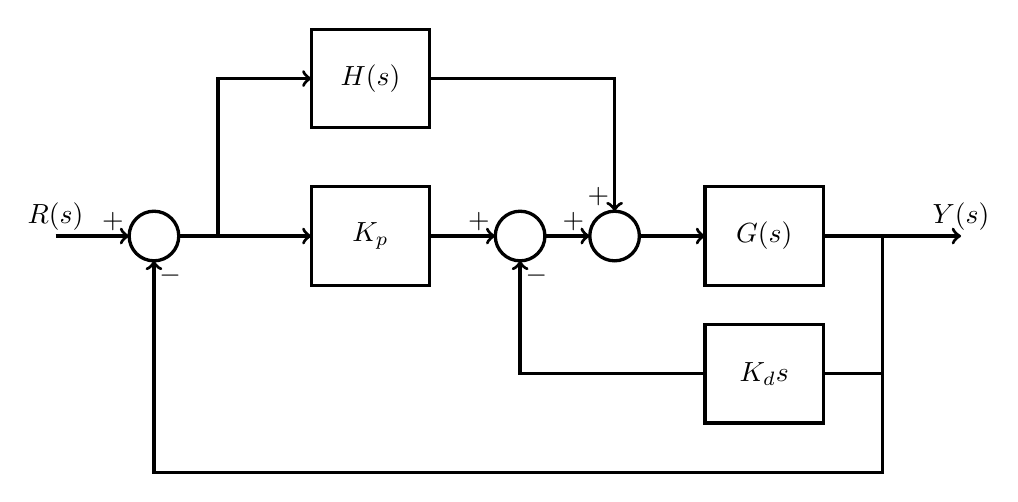
\begin{tikzpicture}[scale=1,inner sep=0pt,outer sep=0pt,very thick,
sysblock/.style={draw,rectangle,inner sep=2pt,minimum width=1.5cm,minimum height=1.25cm,very thick}]

\draw (1.25,0) node[draw,circle] (sum1) {$\rule{0pt}{18pt}$};
\draw (4,0) node[sysblock] (Kp) {$K_{p}$};
%\draw (7,2) node[draw,circle] (sum2) {$\rule{0pt}{18pt}$};
\draw (5.9,0) node[draw,circle] (sum3) {$\rule{0pt}{18pt}$};
\draw (7.1,0) node[draw,circle] (sum4) {$\rule{0pt}{18pt}$};
\draw (9,0) node[sysblock] (G) {$G(s)$};
\draw (9,-1.75) node[sysblock] (Kd) {$K_{d}s$};
\draw (4,2) node[sysblock] (H) {$H(s)$};


\draw[->] (0,0) node[above=2pt] {$R(s)$} -- (sum1.180) node[above left=2pt] {$+$};
\draw[->] (sum1.0) --  (Kp);
\draw[->] (Kp) -- (sum3.180) node[above left=2pt] {$+$};
%\draw[->] (sum3.0) -- node[above=2pt,pos=.4] {$U(s)$}  (sum2.-180) node[above left=2pt] {$+$};
%\draw[->] (sum2.0) -- (G);
\draw[->] (sum3.0) -- (sum4.180) node[above left=2pt] {$+$};
\draw[->] (sum4.0) --  (G);
\draw[->] (G) -- ++(2.5,0) node[above=2pt] {$Y(s)$};
\draw[->] (G) ++(1.5,0) |- (Kd) -| (sum3.-90) node[below right=2pt] {$-$};
\draw[->] (G) ++(1.5,0) -- ++(0,-3) -| (sum1.-90) node[below right=2pt] {$-$};
\draw[->] (H.0) -| (sum4.90) node[above left=2pt] {$+$};
\draw[->] (sum1.0) ++(.5,0) |- (H.180);
%\draw[->] (sum2.-90) -- (sum4.90) node[above right=2pt] {$+$};

%\draw[<-] (sum2.90) node[above right=2pt] {$+$} -- ++(0,1) node[right=2pt] {$D(s)$};
\end{tikzpicture}
\end{center}
